% !TeX root = ../main.tex
% Add the above to each chapter to make compiling the PDF easier in some editors.

 \chapter{Approach}\label{chapter:Approach}
 In this chapter we explain the use cases and requirements to design a context-aware pervasive software framework. Then, we illustrate the  proposed architecture and design following from the concepts introduced in the background chapter and taking into account the challenges and possible solutions shown in the foundation chapter. To recap,  our aim is to design a context-aware pervasive software framework to manage and distribute computations while considering resources, dependencies and networking even with an end-to-end path.

\section{Use Cases}
This section provides real life scenarios targeted by our proposed framework. Requirements are then elicited from the use cases and then the framework implementation and design are evaluated against these requirements. Note that; framework idea is not just to implement these use cases, but to provide the ability to distribute, compose and execute various use cases for context-aware pervasive computing. The use cases are mainly targeted to help human beings, increasing their life quality and preserve the environment. 

\subsection{Smart Cities}
One of the most researched areas in the field of IoT is making our cities more advanced, connected and helpful to human beings and the environment. Researchers and professionals have had many ideas to make use of the context-aware sensor networks that can communicate and act independently whenever the situation needs intervention. We take some examples of the smart cities application and show how they can be implemented using our software framework.

\subsubsection{Smart lighting}

Smart lighting is a use case for automatic control of outdoor lamp posts hence optimizing costs for the governments and enterprises in addition to helping the environment by saving energy \cite{6740844}. The outdoor lighting can be automatically started or closed according to certain circumstances. For example, by lighting up when motion is detected   around it and turning off when there is no further motion, or by detecting natural light  and weather circumstances. Moreover, the lamp posts can be monitored in order to see when a lamp needs replacement.  Further, lamp posts can detect what is the best lighting percentage in a certain situation according to a machine learning algorithm based on the history of decisions taken and feedback provided by users.  In order to implement this use case in our proposed software framework, we must be able to distribute a computational flow to all lamp posts using a messaging system.  Also, the flow should be able to access sensors and be capable of adjusting the light according to the input gathered from several sources including motion, light and humidity sensors.  The decisions taken  should  be   stored into a database so that the flow can access  previous decisions in order to asses the current situation. In addition, a flow with an endpoint that  allows users send feedback on the lighting system can be locally composed to enhance the learning algorithm. Having sent the computational flow to all the lamp posts, the framework should ensure that it does not get deployed on lamp posts without the  required resources, sensors and actuators. 

\subsubsection{Smart Parking}

 which might produce the need for streaming the footage in real-time to other devices.

%\subsubsection{Crowded Subway Cars detection}
%Using the subway as a mean of transportation in the rush hour can be troublesome, most subway cars are crowded in that time. However, in some of the cases, people in the cars are not normally distributed meaning some cars may be less or more crowded than the others. In this sense, people %thought of using cameras, sensors and actuators to signal people for the less crowded cars. 



\subsection{Mining Applications}

In mining fields it is necessary to always monitor gas and temperature levels in order to prevent miners suffocation \cite{doi:10.1155/2013/159273}. At the same time, it is very hard to maintain a connection between sensors in the inside and  monitoring systems outside \cite{ginzboorg2010dtn}. Therefore, the devices incorporated with sensors inside the fields are expected to be pervasive and warn miners from unexpected increase of gas levels on their own. In addition to delivering the data to the outside world, the system must be able to gather data about the situation inside. This requires miners to act as middlemen who store delay-tolerant data into their mobile devices and carry it forward to the outside world. Of course the miners cannot do this process manually, therefore, there should be a messaging system on their mobile devices that carry the data and handle the synchronization with other device. Also, carrying the data in and out is not the only issue, importing and visualizing  data in the monitoring system should be also done automatically.\\

\noindent The mining use case is a delay-tolerant application because there is a big chance there are no wiring going in and out of the mine where new tunnels are constructed thus a delay-tolerant messaging system should be used. But also, it is an information-centric  application because data should be sent data from  devices in the mine to be imported in  the monitoring system without knowing their host names. Having smart devices installed in the mine means its very hard to target them as endpoints without a valid connection, even if there was one, knowing the host names of these devices might still be an issue. Same applies to the monitoring system outside,  data cannot be sent to a specific host name, rather sent to whoever is interested in  these data.

\subsection{Privacy and Security}
The surveillance systems used at the moment upload  tapes, images and footage of people using public transportation to the cloud and then apply facial recognition algorithms in order to  detect faces of wanted criminals. Despite this being of  significant importance to the national security, this puts everyones privacy in jeopardy. Therefore, we thought of replacing this model by a pervasive one, where  the facial detection algorithm and faces of  wanted criminals are pushed to the smart devices in public transportation and whenever a match is found the national security is notified. This helps greatly in increasing privacy, decreasing  latency between the footage and detection in addition to minimizing network bandwidth since the streaming footage  will not be uploaded to the cloud unless there is a match. Similar approaches were introduced in \cite{4653063} and \cite{winkler2010trustcam} where the footage is analyzed on spot to protect privacy. Nevertheless, this is not trivial, facial recognition algorithms are complex and depends on other libraries and  detection models. Therefore, the computation which includes the recognition algorithm  must be able to carry dependencies otherwise the computation will not run. Moreover, the national security should be able to update the list of criminal faces thus messages sent to the smart devices should allow also attachments and dependencies as well. 


\section{Requirements} \label{sec:requirements}

What follows is an enlisting of  the requirements extracted from the real life use cases mentioned in the previous section. We then  evaluate the design and implementation of the framework according to the derived requirements which are  classified  in the following points:
%The framework should
\begin{enumerate}
\item \textit{Service discovery}: since we do not know the host names of the smart devices nor their addresses, the framework should have service discovery mechanism encapsulated in the messaging system as explained in Section \ref{subsec:pub-sub}  to discover peers and  allow any interaction between smart devices.
		
\item \textit{Send and deploy computations}: whatever the use case may be, one of the main requirements of this work, is to be able to send computations to smart devices. This includes sending to one, a set or all smart devices connected together in a network. However, to deploy a computations, the receiving side must have the required hardware resources, sensors and actuators to be qualified for deploying the computation.
 
 \item \textit{Computation dependencies}: complex computations which cannot be executed using the basic operating system and common libraries installed on the smart devices, should carry their  own custom dependencies in order to guarantee a successful run on the receiving smart devices. 


\item \textit{Disconnected devices}: since the framework is also designed to be used in challenged networks, isolated devices in separate networks should also send and receive data or computations using the delay-tolerant architecture.


\item \textit{Communication}: smart devices should be able to communicate, send and receive data in an information-centric and a publish-subscribe manner.

\item \textit{Global identifier}: each smart device must have its own unique global identifier which can be used to send data and computations to this device only.

\item \textit{Composability}: the framework should allow composition of multiple computations either locally through a database or globally by allowing data exchange via the publish-subscribe messaging system.

\item \textit{Pervasiveness}: each computation should be able to act on its own, trigger actuators, persist data and access resources such as cameras and sensors if required by the use case.
\end{enumerate}

\section{Framework Architecture}\label{sec:design}
This section explains the software framework architecture designed for pervasive environments and challenged networks to distribute and manage computations with their respective resources and dependencies.  The main idea behind this design is to harness the features of node-RED to create, deploy and share computations of any kind. In addition to having SCAMPI as an information-centric, publish-subscribe and delay tolerant messaging system that gives the framework the ability to deliver messages even without an end-to-end path. However, node-RED and SCAMPI are two different environments that cannot manage computations, resources and dependencies on their own. They need a middleware to orchestrate the communication between them.\\


\noindent In general the architecture stack on each device should look like Figure \ref{fig:stack}. With SCAMPI at the stack bottom relying only on the JVM. Then on top of SCAMPI is its Java API to communicate with the TCP API of SCAMPI. Afterwards, comes the middleware which acts mediator in between node-RED and SCAMPI. Finally, at the very top exits node-RED to run computations and interact with the user if needed. However, if SCAMPI is used on an android device, there might be no need to run neither the middelware nor node-RED since the phone will be  merely used to transport data from one device to another having no end-to-end path. Below we explain how each component of the system works.
\begin{figure}[H]
	\centering
	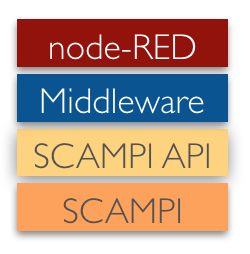
\includegraphics[scale=0.8]{images/stack.png}
	\caption{The framework architecture stack.  }
	\label{fig:stack}
\end{figure}



\subsection{SCAMPI}
As mentioned before SCAMPI is an information-centric, publish-subscribe and delay-tolerant messaging system. In this framework we use SCAMPI to send or receive messages that include computations and data. SCAMPI is also broker-less meaning we do not have to set up a server as broker which is one of the main reasons we chose SCAMPI, in order to be dynamic as possible. The other main reason is to reach devices which do not have direct connectivity to the publishing device or do not have end-to-end path. \\

\noindent Being a delay-tolerant networking architecture, SCAMPI can use its store-carry-forward routing to deliver messages in challenged environments. In figure \ref{fig:scampi-design}, we show how SCAMPI uses mobile phones to connect devices that do not have a route or  direct connection and want to exchange messages. In the figure, there are three Raspberry Pi devices running our proposed stack. The first two  have network connection therefore it is rather easy to exchange messages between themselves. However, the third one is isolated, nevertheless it can be connected to a Wi-Fi network or run as an access point. In this case, an android device passing  between network \textit{N1} and \textit{N2} can carry the message bundles from one network and forward it to the other by connecting to both networks alternatingly.  Thus, reaching out to challenged environments that cannot be reached using wired or wireless connections.

\begin{figure}[H]
	\centering
	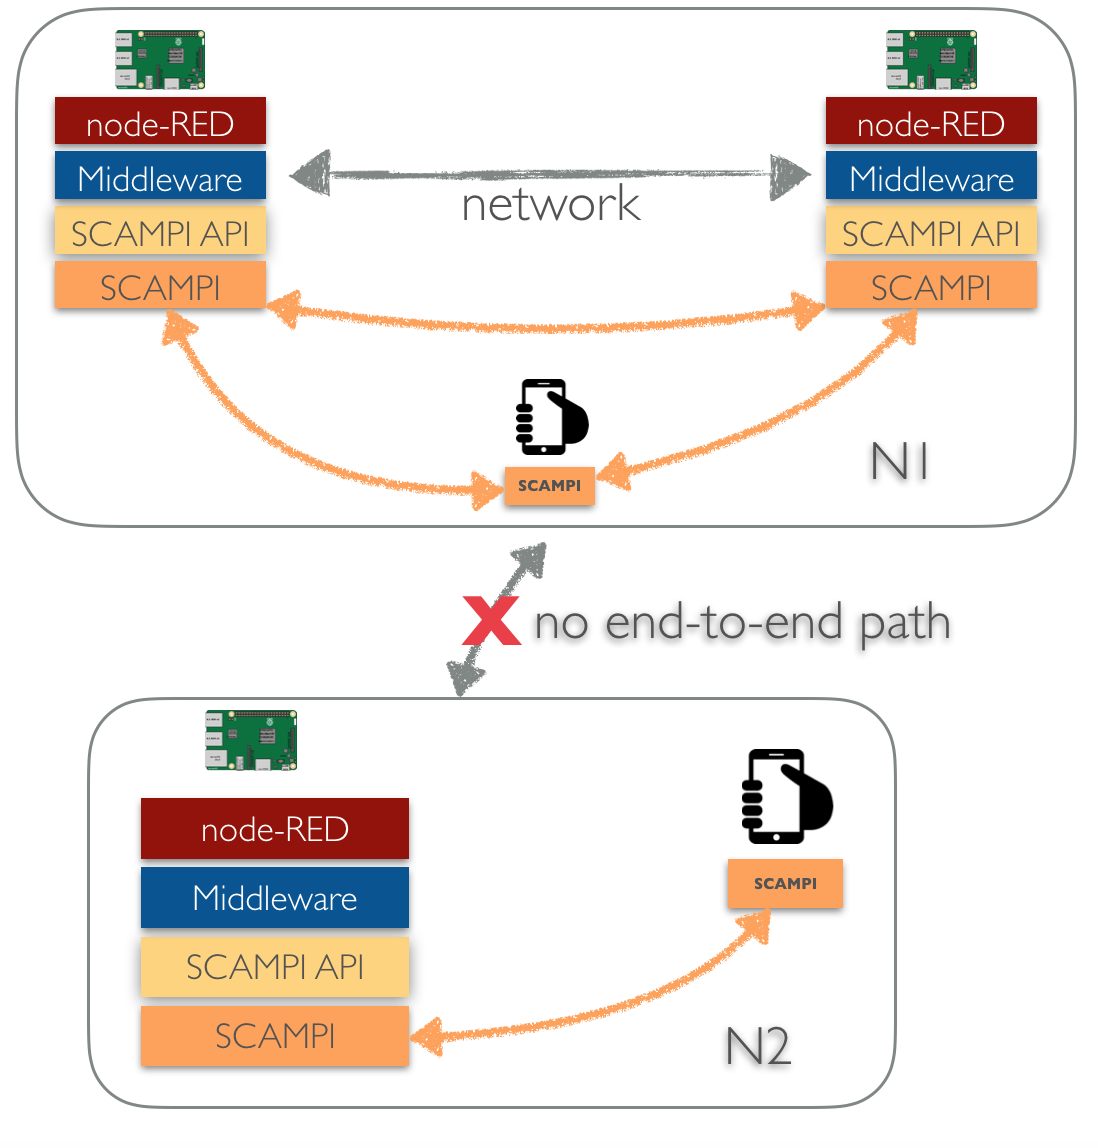
\includegraphics[scale=0.4]{images/scampi.png}
	\caption{SCAMPI synchronization even without an end-to-end path. }
	\label{fig:scampi-design}
\end{figure}

\noindent Being information-centric, data-centric with publish-subscribe pattern and having peer discovery helps us in achieving our dynamic framework without knowing any host names. It  also supports adding and removing devices at will without any additional configuration. We can also use the general identifiers of the devices as topics in order to target each of them independently. As stated, SCAMPI does not have any dependencies other than the JVM so we just run it on each device and we are  good to go. \\


\noindent The SCAMPI Java API acts as a client to the server allowing us to publish or subscribe for any topic from the Java environment. Therefore, we are able to extend this API and create a running Java application that uses the TCP API for SCAMPI underneath. The API also allows the client to override the functions for SCAMPI status changes  for instance if it is disconnected, stopped or most importantly when a new message is received. Furthermore, there is a model called \textit{SCAMPIMessage} used to create messages, it assists in assigning attributes to the message whether strings, integers or even binaries. Also, one can assign meta-data and lifetime to the message.


\subsection{Node-RED}

Node-RED is a tool used for wiring IoT applications, its flows describe the intended computations. It has exporting and importing endpoints for flows via REST which makes it easy to deploy without human interaction.  Flows can be also configured to access certain tables or collections on a running database instance and this configuration can be serialized with the flow. In this framework whenever a flow wants to send a message to another flow on the same node-RED instance or on other instances, it either uses the REST API that the middleware provides to publish and subscribe to data topics or the same database configuration in both flows to be able to communicate data through the database. This allows node-RED to send or receive data and allow composability both locally and globally.  Further, node-RED is rich with predefined nodes that  can be used to run flows on time intervals, connect to emails, twitter accounts or even access a gpio pin on Raspberry Pi. Node-RED usage is intuitive since it is based on flow-programming, it does not need a developer to create a flow:

\subsection{Middleware}
The middleware is this framework's mediator and the main contribution in this work, it is deployed along with node-RED and SCAMPI on each instance in this architecture. It runs a jar file containing a web application server. It has several duties in orchestrating  SCAMPI messages to node-RED instances.
\begin{itemize}
\item It reads the machine specifications to initialize the machine's resources, sensors and actuators 	.
\item It includes the SCAMPI Java API and has a REST API over it which allows any other script from any other language ("including node-RED") to use the publish-subscribe feature of SCAMPI.
\item It analyzes  flows by checking the meta-data  attached to the message thus if the middleware finds out that a flow does not have the necessary hardware requirements, sensors or actuators, it will not deploy the flow. 
\item It is responsible for attaching dependencies of  node-RED flows when one is published, also for putting them into the correct directory when receiving them.
\item It provides a message caching mechanism in order to make sure messages are not handled more than once.
\item it provides a mapping between the topics and node-RED flows meaning if one or more flows are interested in the same topic, all of them should get the data exchanged on this topic.
 \end{itemize}

\subsection{Architecture Usage} \label{subsec:usage}
The following Figure \ref{fig:design} explains how the framework works and shows how data flows between the stack components. In this section, we explain the basic usage of the architecture.

\begin{figure}[H]
	\centering
	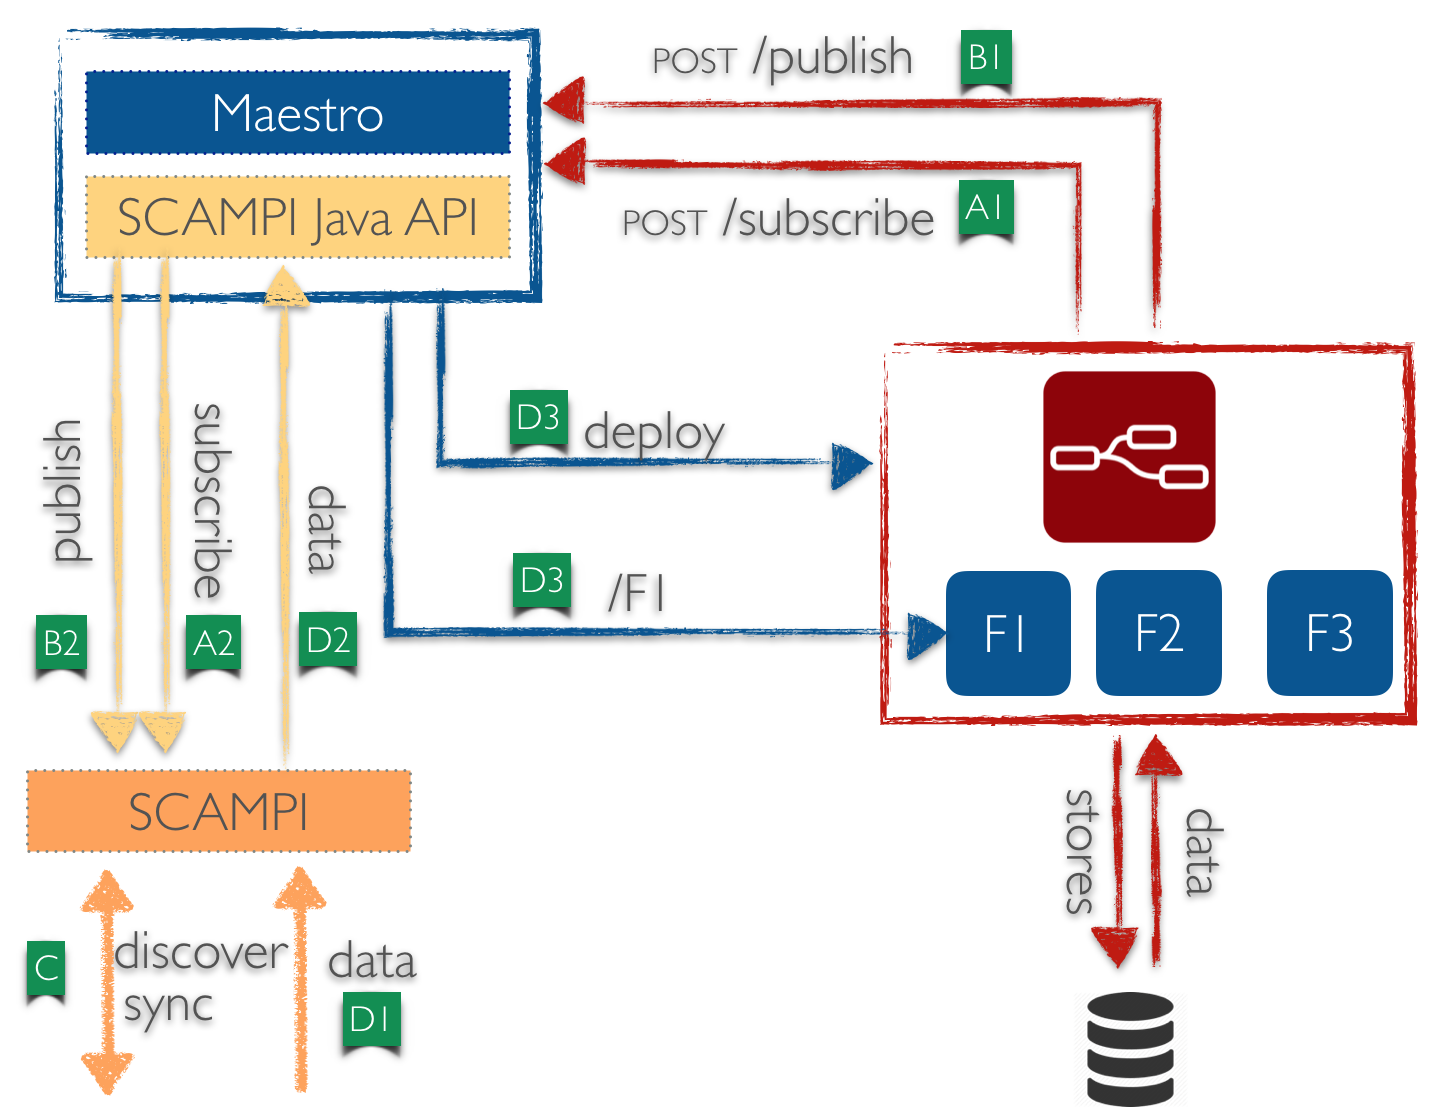
\includegraphics[scale=0.5]{images/design.png}
	\caption{Software framework architecture design. }
	\label{fig:design}
\end{figure}

\begin{enumerate}[label=(\Alph*)]
 
 \item Flows are developed using node-RED UI, they can include publishing and subscribing REST calls to the middleware. If a flow subscribes to a certain topic, the middelware creates  a topic-endpoint mapping between the topic and an endpoint for this flow specifically. Then send a subscribe request to SCAMPI. If another flow on the same instance wants to subscribe to the same topic, the middleware extends the mapping to include it, hence, once a message is received it gets forwarded to all subscribed flow endpoints. 

 \item When the middleware receives a publish request from node-RED, it attaches the dependencies and an indicator that states if the response should be received by the sending device only. Then the message is forwarded to SCAMPI server.

 \item SCAMPI keeps synchronizing messages and discovering new peers continuously as long as its running. Also, storing some message for the store-carry-forward routing functionality.

 \item When a SCAMPI instance receives data it is forwarded to the middleware, which then verifies the topic. If it was a computation then the middleware  checks meta-data, resources, dependencies and then either deploy the computation to node-RED or discard it. Otherwise, if it was a data topic the middleware forward the data to the subscribing flows from the topic-endpoint mapping. 

\end{enumerate}

\section{Summary}

In this chapter we introduced real life use cases for our software framework that was utilized to elicit the requirements used to evaluate the implementation and design of this framework. Afterwards, we described the stack  to implement this framework starting by SCAMPI the  delay-tolerant information-centric messaging system, going through node-RED the platform used to implement, export and execute custom computations serving different use cases, finally we explained the middleware which orchestrates the communication between SCAMPI and node-RED.